
\chapter{\uppercase{The Moment-Based Low-Order Equations}}

The formation of the LO equations is similar to a discontinuous FE method.  Weighted
integrals of the the equations are taken with functions that have local support as weight
functions.  The equations are written with element-wise moments of $I$ and $T$ as
unknowns.  Leaving the solution in this form allows for use of information form a
previous HO solution to eliminate auxillary unknowns from the equations. This is different than a standard Galerkin FE
method~\cite{fe_book} where a
functional form of the solution is directly assumed. The final equations will have a
similar form to S$_2$ equations, but we have not used a collocation method in angle,
which should limit ray effects~\cite{ray_effects} in higher spatial dimensions.
The equations eliminate extra spatial unknowns in a manner similar to to a linear-discontinuous FE
method~\cite{morel_ldtrt}.  We also explore the
possibility of using the MC solution to modify the discretization of the LO solution in
Sec.~\ref{sec:spat_clos}.   MOVE


The remainder of this chapter is structured as follows: the general moments will be
derived and then the angular and spatial closure are discussed REWRITE.  For
simplicity, the backward Euler time discretization is used throughout this section.
Sec.~\ref{sec:time_cont} will use the HO solution and MC transport to consistently
close the equations in time, improving time accuracy.

\section{Forming the Space-Angle Moment Equations}

\subsection{LO Spatial mesh and Finite-Element Spatial Moments}

The LO equations are formulated over a FE mesh.  The domain for the $i$-th spatial
element (or cell) has support $x\in[x_{i-1/2},x_{i+1/2}]$ with width $h_i=x_{i+1/2} -
x_\il$ and cell center 
$x_i = x_\il + h_i/2$.  There is a total of $N_c$ elements, spanning the
spatial domain $0\leq x\leq X$.  For simplicity, this spatial mesh is fixed throughout the
simulation.  Mesh adaptation is only applied in the HO solver.

\begin{figure}[H]
    \centering
    \begin{centering}
        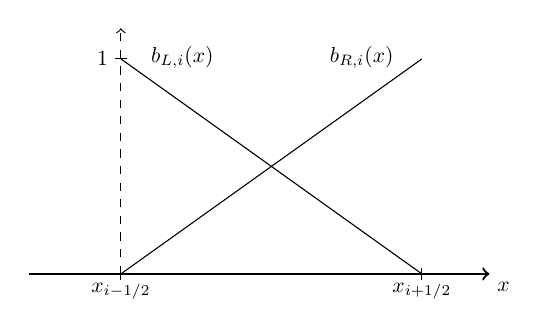
\begin{tikzpicture}[scale=0.78, every node/.style={transform shape}]
            \node at (10.7,4.0) {${1}$  };
            \draw (10.9,4.0) -- (11.1,4.0);
            \draw (11.0,0.4) -- (11.0,0.6) node[below, pos=0.4] {$x_{i-1/2}$};
            \draw (15.90,0.4) -- (15.90,0.6) node[below, pos=0.4] {$x_{i+1/2}$};
            \node at (14.92,4.02) {$b_{R,i}(x)$};
            \node at (12.0,4.02) {$b_{L,i}(x)$};
            \draw [thick,->] (9.5,0.5) -- (17.0,0.5) node[anchor=north west] {$x$};
            \draw [dashed,->] (11.0,0.5) -- (11.0,4.5);
            \draw (11.0,0.5) -- (15.90,4.0);
            \draw (15.90,0.5) -- (11.0,4.0);
        \end{tikzpicture}
    \end{centering}
    \caption{Illustration of linear finite element basis functions $b_{L,i}(x)$ and
    $b_{R,i}(x)$ for spatial element $i$.\label{fig:lin_fe}}
\end{figure}

The spatial moments are defined by integrals weighted with the standard linear finite element (FE)
interpolatory basis functions.  An illustration of the two linear FE basis functions for the $i$-th element is
given in Fig.~\ref{fig:lin_fe}.  The left basis function is defined as
\begin{equation}
    b_{L,i}(x)= \left\{\begin{matrix} \frac{x_\ir - x}{h_i} & x_\il \leq x \leq x_\ir
        \\ 0 &  \text{elsewhere}
    \end{matrix}\right.,
\end{equation}
corresponding to the node $x_\il$.
The right basis function is 
\begin{equation}
    b_{R,i}(x)= \left\{\begin{matrix} \frac{x - x_\il}{h_i} & x_\il \leq x \leq x_\ir
        \\ 0 & \text{elsewhere}
    \end{matrix}\right. ,
\end{equation}
corresponding to the node $x_\ir$. With these definitions, a local linear approximation to a
function $f$ can be formulated as $f(x)\simeq f_{L,i} b_{L,i}(x) + f_{R,i}
b_{R,i}(x),\quad x\in[x_{\il},x_{\ir}]$.\footnote{In literature the FE functions are
formally defined with support over two adjacent elements.  However, in our notation our 
functions only have non-zero support in element $i$. This accommodates our later
definition of moments and discontinuous unknowns.}

The spatial moments are defined by integrals over the each element, using the two
basis functions.  We use $\mom{\cdot}$ to indicate integration over a
spatial element.  The spatial moments are
\begin{equation}\label{eq:x_moml}
\mom{\cdot}_{L,i} = \frac{2}{h_i} \int_{x_{i-1/2}}^{\xr} b_{L,i}(x) (\cdot) \dd x
\end{equation}
and
\begin{equation}\label{eq:x_momr}
\mom{\cdot}_{R,i} = \frac{2}{h_i} \int_{x_{i-1/2}}^{\xr} b_{R,i}(x) (\cdot) \dd x.
\end{equation}
where the factor of $2/h_i$ is a normalization constant.
It is noted in this notation $\mom{\phi}_{L,i}$ and
$\mom{\phi}_{R,i}$ represent spatial moments of the intensity over cell $i$, opposed
to $\phi_{L,i}$ and $\phi_{R,i}$, which represent the interior value of the linear
representation of $\phi(x)$ at $x_\il$ and $x_\ir$ within the cell. 

To simplify notation and discussion, we also define the slope and average moments over a
spatial cell.  The average scalar intensity is
\begin{equation}
    \phi_i = \frac{1}{h_i} \int_{\xl}^{\xr} \phi(x) \dd x
\end{equation}
and
\begin{equation}
    \phi_{x,i} = \frac{6}{h_i} \int_{\xl}^{\xr} \left(\frac{x-x_i}{h_i} \right)
    \phi(x) \dd x . 
\end{equation}
The linear representation over a cell in terms of these moments is $\phi(x) = \phi_i
+ 2\phi_{x,i}(x - x_i)/h_i^2$, for $x\in(\xl,\xr)$. 

\subsection{Definition of Angular Moments}

To reduce the angular dimensionality, positive and
negative half-range integrals of the angular intensity are taken.  The angular integrals
are denoted with a superscript as
\begin{equation}
    (\cdot)^\pm =  \pm\int_0^{\pm1} (\cdot) \dd \mu
\end{equation}
The half-range
integrals of $I$ are defined as $ \phi^+(x,t) = \int_0^{1} I(x,\mu,t)\, \dd \mu$ and $
\phi^-(x,t) = 2 \pi \int_{-1}^{0} I(x,\mu,t) \,\dd
\mu$, respectively.  Thus, in terms of half-range quantities, the mean intensity is $\phi = \phi^- +
\phi ^+$.  It is noted that in this notation the flux is defined as
$J=J^-+J^+$, which is not the standard definition for the half-range fluxes, e.g.,
in~\cite{lewis}.

\subsection{Space-Angle Moments of the Radiation Transport Equation}

The LO radiation equations are formed by applying the space and angle moment operators to the
transport equation and performing algebraic manipulation.  We provide a detailed
derivation of the $L$ and $+$ radiation moment equation and state the final results for the
other moment operators.  First, the $L$ moment operator is applied to the time-discretized transport equation,
i.e., Eq.~\eqref{eq:trans_td}.  Integration by parts on the streaming term yields
\begin{multline}
    -\frac{2}{h_i}{\mu}_{i-1/2} I_{i-1/2}^{n+1} + \frac{2}{h_i^2}\int_{\xl}^{\xr} \mu I^{n+1} \dd x
        +  \left(\sigma_{t,i}^{n+1}+\frac{1}{c \Delta t} \right)  
        \mom{\phi}_{L,i}^{n+1,+} \\-  \frac{\sigma_{s,i} }{2} \mom{\phi}_{L,i}^{n+1} =
        \frac{1}{2} \mom{\sigma_a^{n+1} a c T^{n+1,4}}_{L,i} +
  \frac{1}{c\Delta t}\mom{\phi}_{L,i}^{n,+}.
\end{multline}
Here, the cross sections have been assumed constant over a cell.  The mean
intensity in the scattering term is expanded in terms of half-range unknowns.
The integral can be rewritten in terms of $L$ and $R$ moments by noting that $b_{L,i}(x) +
b_{R,i}(x) = 2/h_i$.  These substitutions are made and the resulting equation is
multiplied by $h_i$ to produce
\begin{multline}
    -2{\mu}_{i-1/2} I_{i-1/2}^{n+1} + \mom{\mu I^{n+1}}_{L,i} + \mom{\mu I^{n+1}}_{R,i} 
        +  \left(\sigma_{t,i}^{n+1}+\frac{1}{c \Delta t} \right) h_i 
  \mom{\phi}_{L,i}^{n+1,+} \\-  \frac{\sigma_{s,i} h_i}{2} \left( \mom{\phi}_{L,i}^{n+1,+} +
  \mom\phi_{L,i}^{n+1,-}\right) = \frac{h_i}{2} \mom{\sigma_a^{n+1} a c T^{n+1,4}}_{L,i} +
  \frac{h_i}{c\Delta t}\mom{\phi}_{L,i}^{n,+}.
\end{multline}
The resulting equation is integrated over the positive half range:
\begin{multline}\label{eq:spat_mom}
    -2\left({\mu}_{i-1/2} I_{i-1/2}^{n+1}\right)^+ + \mom{\mu I^{n+1}}^+_{L,i} + \mom{\mu
        I^{n+1}}^+_{R,i} 
        +  \left(\sigma_{t,i}^{n+1}+\frac{1}{c \Delta t} \right) h_i 
  \mom{\phi}_{L,i}^{n+1,+} \\-  \frac{\sigma_{s,i} h_i}{2} \left( \mom{\phi}_{L,i}^{n+1,+} +
  \mom\phi_{L,i}^{n+1,-}\right) = \frac{h_i}{2} \mom{\sigma_a^{n+1} a c T^{n+1,4}}_{L,i} +
  \frac{h_i}{c\Delta t}\mom{\phi}_{L,i}^{n,+}.
\end{multline}

\subsection{The Angular Consistency Terms}

Now, algebraic manipulations are performed on the streaming terms to produce face and
volume-averaged values of $\mu$, weighted by the intensity.  Each term in the streaming
term is multiplied by a factor of unity, with the desired unknown appropriate to each term
in the numerator and denominator.  Temporarily dropping the time
index for clarity, the manipulations applied to
the streaming term are as follows:
    \begin{align} \label{eq:line1}
        {\displaystyle \left \langle \mu \pderiv{I}{x} \right \rangle_L^+ } & = 
        -\frac{\ds2}{\ds h_i} \left(\mu I_{i-1/2}\right)^+ + \frac{\ds 1}{\ds h_i}\left[
    \mom{\mu I}_{L,i}^+ + \mom{\mu I}_{R,i}^+ \right] \\
        & =  
        -\frac{\ds2}{\ds h_i} \left(\mu I_{i-1/2}\right)^+
        \! \frac{\ds(I_{i-1/2})^+}{\ds(I_{i-1/2})^+}  \;    + \frac{\ds 1}{\ds h_i}\left[ \;
        \mom{\mu I}_{L,i}^+ \! \frac{\ds\mom{I}_{L,i}^+}{\ds\mom{I}_{L,i}^+} \; + \; \mom{\mu
        I}_{R,i}^+ \! \frac{\ds\mom{I}_{R,i}^+}{\ds\mom{I}_{R,i}^+} \right] \\
        & =  -\frac{\ds2}{\ds h_i} \left\{ {\frac{\ds \left( \mu I
            \right)^+_{i-1/2} }{\ds\phi^+_{i-1/2}}} \right\}
            \phi^+_{i-1/2} + \frac{\ds 1}{\ds h_i} \left[ \left\{ {\frac{\ds\mom{\mu
        I}_{L,i}^+}{\ds\mom{\phi}_{L,i}^+}} \right \} \mom{\phi}_{L,i}^+  +
        \left\{ {\frac{\ds\mom{\mu I}_{R,i}^+}{\ds\mom{\phi}_{R,i}^+}} \right\}
    \mom{\phi}_{R,i}^+ \right]
    \end{align}
The ratios in braces are what we will formally define as \emph{angular consistency terms}.
These nonlinear functionals are approximated by the HO solver.  The angular consistency
term for the $L$ and $+$ moments is defined as
\begin{equation}\label{eq:ang_cons_vol}
    \cur{{\mu}}_{L,i}^{n+1,+} \equiv \frac{\mom{\mu I^{n+1}}_{L,i}^+}{\mom{I^{n+1}}_{L,i}^+} =  \frac{
{\displaystyle \frac{2}{h_i}} \int\limits_0^1 \int\limits_\xl^\xr \mu \, b_{L,i}(x)
I^{n+1}(x,\mu) \dd x \dd \mu } 
{{\displaystyle \frac{2}{h_i}} \int\limits_0^1 \int\limits_\xl^\xr \, b_{L,i}(x)
I^{n+1}(x,\mu) \dd x \dd \mu } .
\end{equation}
The consistency terms on the face represent averaging at a point, with a similar
definition as
\begin{equation}\label{eq:ang_cons_face}
    {\mu}_{i+1/2}^{+} \equiv \frac{\left(\mu I_{i+ 1/2}\right)^+}{\phi_{i+1/2}^+}=  \frac{
        {\displaystyle \int\limits_0^1 \mu I(x_{i+1/2},\mu) \dd \mu }} 
        {{\displaystyle \int\limits_0^1 I(x_{i+1/2},\mu) \dd \mu }} \;.
\end{equation}
There are analogous definitions for the $R$ and $-$ moments.
The moment of the streaming
term for the $L$ and $+$ operators becomes
\begin{equation}\label{eq:stream_mom}
        {\displaystyle \left \langle \mu \pderiv{I}{x} \right \rangle_L^+ } = 
        -\frac{\ds2}{\ds h_i} \mu_{i-1/2}^+ I_{i-1/2}^+ + \frac{1}{h_i}\left[
        \cur{\mu}_{L,i}^+ \mom{\phi}^+_{L,i} + \cur{\mu}_{R,i}^+ \mom{\phi}_{R,i}^+
    \right]
\end{equation}


\subsection{The Exact Radiation Moment Equations}

A final expression for the moment equation resulting from application of the $L$ moment and
positive half-range integral is obtained by substituting the result of
Eq.~\eqref{eq:stream_mom} into Eq.~\eqref{eq:spat_mom}:
\begin{multline}\label{eq:exact_lmomp}
    -2{\mu}_{i-1/2}^{n+1,+} \phi_{i-1/2}^{n+1,+} + \cur {\mu}_{L,i}^{n+1,+}
  \mom{\phi}_{L,i}^{n+1,+}
  +  \cur\mu_{R,i}^{n+1,+}
  \mom{\phi}_{R,i}^{n+1,+} +  \left(\sigma_{t,i}^{n+1}+\frac{1}{c \Delta t} \right) h_i 
  \mom{\phi}_{L,i}^{n+1,+} \\-  \frac{\sigma_{s,i} h_i}{2} \left( \mom{\phi}_{L,i}^{n+1,+} +
  \mom\phi_{L,i}^{n+1,-}\right) = \frac{h_i}{2} \mom{\sigma_a^{n+1} a c T^{n+1,4}}_{L,i} +
  \frac{h_i}{c\Delta t}\mom{\phi}_{L,i}^{n,+},
\end{multline}
Similar derivations can be used to derive the other radiation moment equations.  
Pairwise application of the $L$ and $R$ basis
moments with the $+$ and $-$ half-range integrals to Eq.~\eqref{ho_trans} 
ultimately yields four moment
equations per cell.  The equation for the $R$ and $+$ moment is
\begin{multline}\label{eq:exact_rmomp}
    2{\mu}_{i+1/2}^{n+1,+} \phi_{i+1/2}^{n+1,+} - \cur {\mu}_{L,i}^{n+1,+}
  \mom{\phi}_{L,i}^{n+1,+}
  -  \cur\mu_{R,i}^{n+1,+}
  \mom{\phi}_{R,i}^{n+1,+} +  \left(\sigma_{t,i}^{n+1}+\frac{1}{c \Delta t} \right) h_i 
  \mom{\phi}_{R,i}^{n+1,+} \\-  \frac{\sigma_{s,i} h_i}{2} \left( \mom{\phi}_{R,i}^{n+1,+} +
  \mom\phi_{R,i}^{n+1,-}\right) = \frac{h_i}{2} \mom{\sigma_a^{n+1} a c T^{n+1,4}}_{R,i} +
  \frac{h_i}{c\Delta t}\mom{\phi}_{R,i}^{n,+},
\end{multline}
The equations for the negative half-range moment are identical to the above with the
negative half-range superscripts replacing the positive.  Explicitly,
\begin{multline}\label{eq:exact_lmomp}
    -2{\mu}_{i-1/2}^{n+1,-} \phi_{i-1/2}^{n+1,-} + \cur {\mu}_{L,i}^{n+1,-}
  \mom{\phi}_{L,i}^{n+1,-}
  +  \cur\mu_{R,i}^{n+1,-}
  \mom{\phi}_{R,i}^{n+1,-} +  \left(\sigma_{t,i}^{n+1}+\frac{1}{c \Delta t} \right) h_i 
  \mom{\phi}_{L,i}^{n+1,-} \\-  \frac{\sigma_{s,i} h_i}{2} \left( \mom{\phi}_{L,i}^{n+1,+} +
  \mom\phi_{L,i}^{n+1,-}\right) = \frac{h_i}{2} \mom{\sigma_a^{n+1} a c T^{n+1,4}}_{L,i} +
  \frac{h_i}{c\Delta t}\mom{\phi}_{L,i}^{n,-}
\end{multline}
and
\begin{multline}\label{eq:exact_rmomp}
    2{\mu}_{i+1/2}^{n+1,-} \phi_{i+1/2}^{n+1,-} - \cur {\mu}_{L,i}^{n+1,-}
  \mom{\phi}_{L,i}^{n+1,-}
  -  \cur\mu_{R,i}^{n+1,-}
  \mom{\phi}_{R,i}^{n+1,-} +  \left(\sigma_{t,i}^{n+1}+\frac{1}{c \Delta t} \right) h_i 
  \mom{\phi}_{R,i}^{n+1,-} \\-  \frac{\sigma_{s,i} h_i}{2} \left( \mom{\phi}_{R,i}^{n+1,+} +
  \mom\phi_{R,i}^{n+1,-}\right) = \frac{h_i}{2} \mom{\sigma_a^{n+1} a c T^{n+1,4}}_{R,i} +
  \frac{h_i}{c\Delta t}\mom{\phi}_{R,i}^{n,-},
\end{multline}
Ultimately, the two half-ranges will be treated differently when the equations are closed
spatially.

\subsection{Material Energy Equations}

To derive the LO material energy equations, an approximation must be introduced to relate
$T(x)$ and $T^4(x)$ within a cell.  We represent $T(x)$ spatially 
with a LDFE trial space.  This trial space will ensure preservation of the equilibrium
diffusion limit.  To simplify the relation between $T(x)$ and $T^4(x)$ 
$ T(x) \simeq T_{L,i} b_{L,i}(x) + T_{R,i} b_{R,i}(x),\quad x\in(x_{i-1/2},x_\ir)$.
Similarly, the emission term is represented in the material and radiation equations with the LDFE
interpolant $T^4(x)\simeq T_{L,i}^4 b_{L,i}(x) + T_{R,i}^4 b_{R,i}(x)$.   The $L$ and $R$ spatial moments are taken of the material
energy equations; the LDFE representations for $T(x)$ and $\sigma_a a c T^4(x)$ are used to
simplify the spatial integrals. The final LO material energy
 equation resulting from application of the $L$ moment is
 \begin{multline}\label{lo_mat_dis}
     \frac{\rho_i c_{v,i}}{\Delta t}\left[ \left(\frac{2}{3}T_{L,i} + \frac{1}{3}T_{R,i}
        \right)^{n+1} - \left(\frac{2}{3}T_{L,i} + \frac{1}{3}T_{R,i}
    \right)^{n} \right]  + \sigma_{a,i}^{n+1} \left( \mom{\phi}_{L,i}^+ +
    \mom{\phi}_{L,i}^- \right)^{n+1} \\ = \sigma_{a,i}^{n+1}a c
\left( \frac{2}{3} T_{L,i}^4 + \frac{1}{3}T_{R,i}^4
        \right)^{n+1}.
\end{multline}
The equation for the $R$ moment is
 \begin{multline}\label{lo_mat_dis}
     \frac{\rho_i c_{v,i}}{\Delta t}\left[ \left(\frac{1}{3}T_{L,i} + \frac{2}{3}T_{R,i}
        \right)^{n+1} - \left(\frac{1}{3}T_{L,i} + \frac{2}{3}T_{R,i}
    \right)^{n} \right]  + \sigma_{a,i}^{n+1} \left( \mom{\phi}_{R,i}^+ +
    \mom{\phi}_{R,i}^- \right)^{n+1} \\ = \sigma_{a,i}^{n+1}a c
\left( \frac{1}{3} T_{L,i}^4 + \frac{2}{3}T_{R,i}^4
        \right)^{n+1}.
\end{multline}
Cross sections have been assumed constant over each element, evaluated at the
average temperature within the element, i.e., $\sigma_{a,i}^{n+1} =
\sigma_{a,i}([T^{n+1}_{L,i}+T^{n+1}_{R,i}]/2)$.
Because the material energy balance
 only contains angularly integrated quantities, there is no need to take angular
 moments of the above equations.  

REWRITE: WHAT TO DO WITH THIS PARAGRAPH?
Because there are no derivatives of $T$ in Eq.~\eqref{lo_mat}, there is no need
to define $T$ on the faces.  Because only moments of $\phi$ appear in the material energy
equations, they are fully defined at this point.  The LD closure for the $L$ and $+$ equations produces


\section{Closing the LO System with Information from the HO Solution}
\label{sec:closure}

The six degrees of freedom (DOF) over each cell $i$ are the four moments $\mom{\phi}_{L,i}^+$,
$\mom{\phi}_{R,i}^+$, $\mom{\phi}_{L,i}^-$, and $\mom{\phi}_{R,i}^-$ and the two
spatial edge values $T_{L,i}$ and $T_{R,i}$. The four radiation and two material
energy equations define a system of equations for the six DOF, coupled spatially through
the streaming term.  We emphasize that at this point we have not made any spatial or
angular approximations to the transport moment equations; these moment equations are exact with
respect to the chosen time discretization.  The material energy equation has the
approximation of an LDFE space for $T(x)$.  Some approximation of this form is necessary
to relate $T$ and $T^4$.

\subsection{Angular Closure}

The angular consistency
parameters (e.g., Eq.~\eqref{eq:ang_cons_vol} and~\eqref{eq:ang_cons_face}) are not known a priori. 
A lagged estimate of $I^{n+1}$ from the previous HO solve is
used to estimate the angular consistency parameters. In the HOLO algorithm, the equations for LO unknowns at iteration $k+1$ use consistency parameters
computed using the latest HO solution $\tilde{I}^{n+1,k+1/2}$
as an approximation for $I^{n+1}(x,\mu)$.  We evaluate these terms using quadruature based
on the functional form of the solution provided by the HO solution.

\subsection{Spatial Closure}

The relation between the volume and face averaged quantities must be known to eliminate
the final auxillary unknowns.
To close the LO system spatially, we will explore multiple options.  The simplest closure
is to use a linear-discontinuous (LD) spatial closure with the usual upwinding
approximation~\cite{morel_ldtrt}.  For example, for positive flow (e.g., Eq.~\eqref{eq:lo_tran}) the face terms $\mu_{i-1/2}$ and $\phi_{i-1/2}$
are upwinded from the previous cell $i-1$ or from a boundary condition; the terms
at $x_{i+1/2}$ are linearly extrapolated, computed using the $L$ and $R$ basis
moments.  By assuming $\phi^\pm(x)$ is linear over a cell, a relation between the 
outflow and moments can be derived, e.g., $\phi^+_{i+1/2} = 2\mom{\phi}_R^+ -
\mom{\phi}_L^+$. For the negative half range, $\phi^-_{i-1/2} = 2\mom{\phi}_L^- -
\mom{\phi_R}^+$.  The LD closure, with upwinding, for the $L$ equation and positive half-range is
\begin{equation}
    -2{\mu}_{i-1/2}^{n+1,+} \left(2\mom{\phi}_{R,i-1}^+ -         \right) + \cur {\mu}_{L,i}^{n+1,+}
  \mom{\phi}_{L,i}^{n+1,+}
  +  \cur\mu_{R,i}^{n+1,+}
  \mom{\phi}_{R,i}^{n+1,+} +  \left(\sigma_{t,i}^{n+1}+\frac{1}{c \Delta t} \right) h_i 
  \mom{\phi}_{L,i}^{n+1,+} \\-  \frac{\sigma_{s,i} h_i}{2} \left( \mom{\phi}_{L,i}^{n+1,+} +
  \mom\phi_{L,i}^{n+1,-}\right) = \frac{h_i}{2} \mom{\sigma_a^{n+1} a c T^{n+1,4}}_{L,i} +
  \frac{h_i}{c\Delta t}\mom{\phi}_{L,i}^{n,+}.
\end{equation}
Similar equations can be derived for the other directions, fully defining the radiation
equations. These equations are equivalent to an $S_2$

Note that we have chosen to leave $\mu_{i-1/2}^{n+1,+}$ as a value to be estimated from the HO solver,
which is more conducive to the other spatial closures described in
Sec.~\ref{sec:spat_close}.
Alternatively, the spatial closure could be introduced before performing the algebraic
manipulation to form consistency terms (e.g., into Eq.~\eqref{eq:line1}).  This would produce only volume-weighted consistency
terms for the LD spatial closure.

The choice of a LD spatial closure preserves the equilibrium diffusion limit.  In this limit, the MC HO solution will estimate angular consistency terms 
associated with an isotropic intensity, based on a spatially LD emission source.  The isotropic-intensity consistency terms will produce
LO equations that are equivalent to $S_2$ equations, with quadrature points of $\pm 1/2$.  Because the spatial
closure produces equations that are equivalent to an LDFE solution to these equations, we expect the equations to preserve the
equilibrium diffusion limit~\cite{morel_ldtrt,densmore_edl}.

\subsubsection{Fixups to LD Solution}

The linear-discontinuous (LD) closure with upwinding is not strictly positive.  In particular, for
optically thick cells with a steep intensity gradient, the solution becomes negative.
These negative values of intensity can propagate to adjacent cells. In thick regions of
TRT problems, reasonably fine spatial cells can still be on the order of millions of mean
free paths; negative values with an LD representation are unavoidable in practice for
such cells and mesh refinement is of minimal use.  Typically, for a standard LDFE method,
the equations are lumped to produce a strictly positive solution (for 1D)~\cite{morel_ldtrt}. However, standard FE lumping
procedures would introduce difficulties in computing the consistency terms from the
HO solution.  Thus, an alternative spatial closure is used that is equivalent to the
standard FE lumping procedure.  The $L$ and $R$ moments are defined the same as before,
preserving the average within a cell, but the relation between the moments and
the outflow is modified.   For example, for positive $\mu$,
the outflow is now defined as $\phi^+_{i+1/2} = \mom{\phi}_R^+.$  Because the basis function $b_{R,i}(x)$ is strictly
positive, the outflow is positive.  This closure is only used
in cells where negative intensities occur.

\subsection{Newton's Method for LO Equations}

Adding the equations for each cell together forms a global system of coupled equations.
The equations are nonlinear due to the Planckian emission source.  
We have used Newton's method to solve the nonlinear system, based on a typical linearization of the Planckian source with cross
sections evaluated at temperatures from the previous iteration, as described
in~\cite{morel_ldtrt}.  A derivation of the LO Newton equations is given
in~\ref{app:lo_newton}.

The equations for each half-range are coupled together via scattering.  
In one spatial dimension, the scattering terms can be included in the discrete system
matrix and directly inverted.  We consider an alternative iterative solution method that
could be more easily extended to higher spatial dimensions in Sec.~\ref{sec:dsa}.
Isotropic scattering,
including effective scattering terms from the linearization, are included in the system matrix. The system
matrix is an asymmetric, banded matrix with a band width of seven and is inverted
directly. 
Newton iterations are repeated until $\phi^{n+1}(x)$ and $T^{n+1}(x)$ are converged
to a desired relative tolerance.  Convergence is calculated using the spatial $L_2$
norm of the change in $\phi^{n+1}(x)$ and $T^{n+1}(x)$, relative to the norm of each
solution.  The lumping-equivalent discretization
discussed above is used for cells where the solution for
$\phi^{n+1}$ becomes negative. When negative values for $\phi^{n+1,\pm}(x)$ are detected, the lumping-equivalent discretization is used within
those cells and that Newton step is repeated. 


%Application of the first order Taylor expansion in time of the
%gray emission source, about some temperature $T^*$ at some
%time near $t^{n+1}$ gives
%\begin{equation}\label{new_planck}
%    \sigma_a^* a c T^{4,n+1} \simeq \sigma_a^* a c \left[T^{*4} + (T^{n+1} - T^*) 4T^{*3} \right]
%\end{equation}
%where the superscript $*$ denotes evaluation at $T^*$. A spatially discretized form
%of this expression is substituted
%into the emission term in the discretized material
%energy equations, e.g., Eq.~\eqref{lo_mat_dis}.  This allows for the material energy
%equation to be eliminated from the system, introducing effective scattering and
%emission sources into the right hand side
%of the LO radiation equations. This defines four linear equations for the four remaining radiation unknowns. 
%Once these linear equations have been solved for $\phi^{n+1}$, a new estimate of
%$T^{n+1}$ can be determined using the same linearization (Eq.~\eqref{new_planck}) to
%conserve the total energy.  This estimate of $T^{n+1}$ can now be used as $T^*$ to form a more
%accurate linearization of the emission source. 
